\section{Chapter 9 Implementation and Technology Stack}

\subsection{9.1 Project Structure}

The CloudSentinel AI project is organized to ensure modularity, maintainability, and scalability. The project structure follows a standard software engineering pattern:

\begin{verbatim}
cloudsentinel-ai/
|-- backend/
|   |-- api/
|   |-- auth/
|   |-- collectors/
|   |-- analyzers/
|   |-- graph/
|   |-- attack_engine/
|   |-- risk_engine/
|   |-- ai/
|   |-- reports/
|   |-- database/
|-- frontend/
|   |-- dashboard/
|   |-- components/
|   |-- pages/
|   |-- services/
|-- infrastructure/
|   |-- docker/
|   |-- terraform/
|   |-- aws/
|-- docs/
|-- tests/
|-- README.md
\end{verbatim}

This structure clearly separates business logic, APIs, infrastructure, documentation, and testing, making the project easier to maintain and extend.

\subsection{9.2 Backend Technology Stack}

The backend of CloudSentinel AI is developed using Python, leveraging the FastAPI framework. FastAPI was selected for its high performance, native support for asynchronous programming, and automated data validation features. It provides an efficient platform for handling high-concurrency requests, which is essential for scanning large cloud environments and processing complex graph-based queries.

\subsection{9.3 Frontend Development}

The frontend is built using React.js to provide a responsive, intuitive interface for security analysts. To handle the complex visualization of cloud attack graphs, the dashboard integrates specialized libraries such as Cytoscape.js or D3.js. These tools enable the rendering of interactive nodes and edges, allowing users to zoom, pan, and filter attack paths dynamically.

\subsection{9.4 Database and Data Modeling}

The framework employs a hybrid data storage strategy:

\begin{itemize}
\tightlist
\item
  \textbf{PostgreSQL:} Serves as the primary relational database for storing persistent configuration data, user information, audit logs, and scan history.\\
\item
  \textbf{NetworkX:} Used for in-memory graph construction and algorithm execution during analysis.\\
\item
  \textbf{Graph Database (Future):} While currently utilizing in-memory structures for agility, the architecture is designed to integrate graph-native databases like Neo4j or Amazon Neptune as the environment scale increases.
\end{itemize}

\subsection{9.5 AI and LLM Integration}

The Explainable AI module integrates with Large Language Models (LLMs) through secure API interfaces. The backend processes raw graph data and rule violations, structures them into a context-rich prompt, and sends them to the LLM. The model is specifically tuned through prompt engineering to return standardized, actionable security reports, minimizing hallucinations and ensuring technical accuracy.

\subsection{9.6 Infrastructure and DevOps}

Infrastructure is managed using containerization and Infrastructure-as-Code (IaC) principles:

\begin{itemize}
\tightlist
\item
  \textbf{Docker:} Ensures consistent deployment environments across development, staging, and production by bundling all dependencies.\\
\item
  \textbf{Terraform:} Facilitates the automated provisioning of the infrastructure stack, ensuring scalability, environmental reproducibility, and consistent management of cloud resources.
\end{itemize}

\subsection{9.7 API Design and Documentation}

The application follows RESTful API design principles to ensure a clean interface between the backend engines and the frontend dashboard. All endpoints are secured with JSON Web Token (JWT) authentication, ensuring that only authorized users can trigger scans or view sensitive security findings. The API is documented using the OpenAPI (Swagger) specification, providing clear endpoint definitions and enabling seamless integration for future development.

\subsection{9.8 Security Considerations}

To ensure secure operation, the implementation incorporates several security measures:

\begin{itemize}
\tightlist
\item
  \textbf{Secure Credential Storage:} Utilization of IAM roles or AWS Secrets Manager to manage sensitive credentials.\\
\item
  \textbf{Encrypted Communication:} Enforcement of HTTPS for all client-server communication.\\
\item
  \textbf{Access Control:} Implementation of Role-Based Access Control (RBAC) for all dashboard users.\\
\item
  \textbf{Cryptographic Security:} Password hashing using secure cryptographic algorithms.\\
\item
  \textbf{Auditability:} Comprehensive audit logging for all scan operations.\\
\item
  \textbf{Input Sanitization:} Strict input validation and API request sanitization to prevent injection attacks.\\
\item
  \textbf{Traffic Control:} Rate limiting applied to public endpoints to mitigate denial-of-service risks.\\
\item
  \textbf{Data Protection:} Secure handling of AI-generated reports to prevent sensitive data leakage.
\end{itemize}

\subsection{9.9 Scalability and Future Enhancements}

The modular implementation enables future expansion without significant architectural changes. Potential enhancements include:

\begin{itemize}
\tightlist
\item
  \textbf{Multi-Cloud Support:} Extending coverage to Azure and GCP.\\
\item
  \textbf{Kubernetes Security:} Integration of container and orchestration-level security analysis.\\
\item
  \textbf{IaC Scanning:} Automated security validation for Infrastructure-as-Code templates.\\
\item
  \textbf{Real-time Monitoring:} Implementation of event-driven monitoring using cloud-native triggers.\\
\item
  \textbf{Compliance Automation:} Continuous, automated compliance assessment frameworks.\\
\item
  \textbf{SIEM Integration:} Data export capabilities for Security Information and Event Management platforms.\\
\item
  \textbf{Automated Remediation:} Development of guided or automated remediation workflows.
\end{itemize}

\subsection{9.10 Chapter Summary}

This chapter described the implementation design and technology stack of CloudSentinel AI. It explained the rationale behind the selected technologies, the deployment architecture, the hybrid relational and graph data model, the REST API design, the project structure, and the security considerations that guide the implementation. The proposed implementation emphasizes modularity, scalability, and maintainability while providing a practical roadmap for developing the CloudSentinel AI framework.

\subsection{Additional Figures}

\begin{figure}[H]
\centering
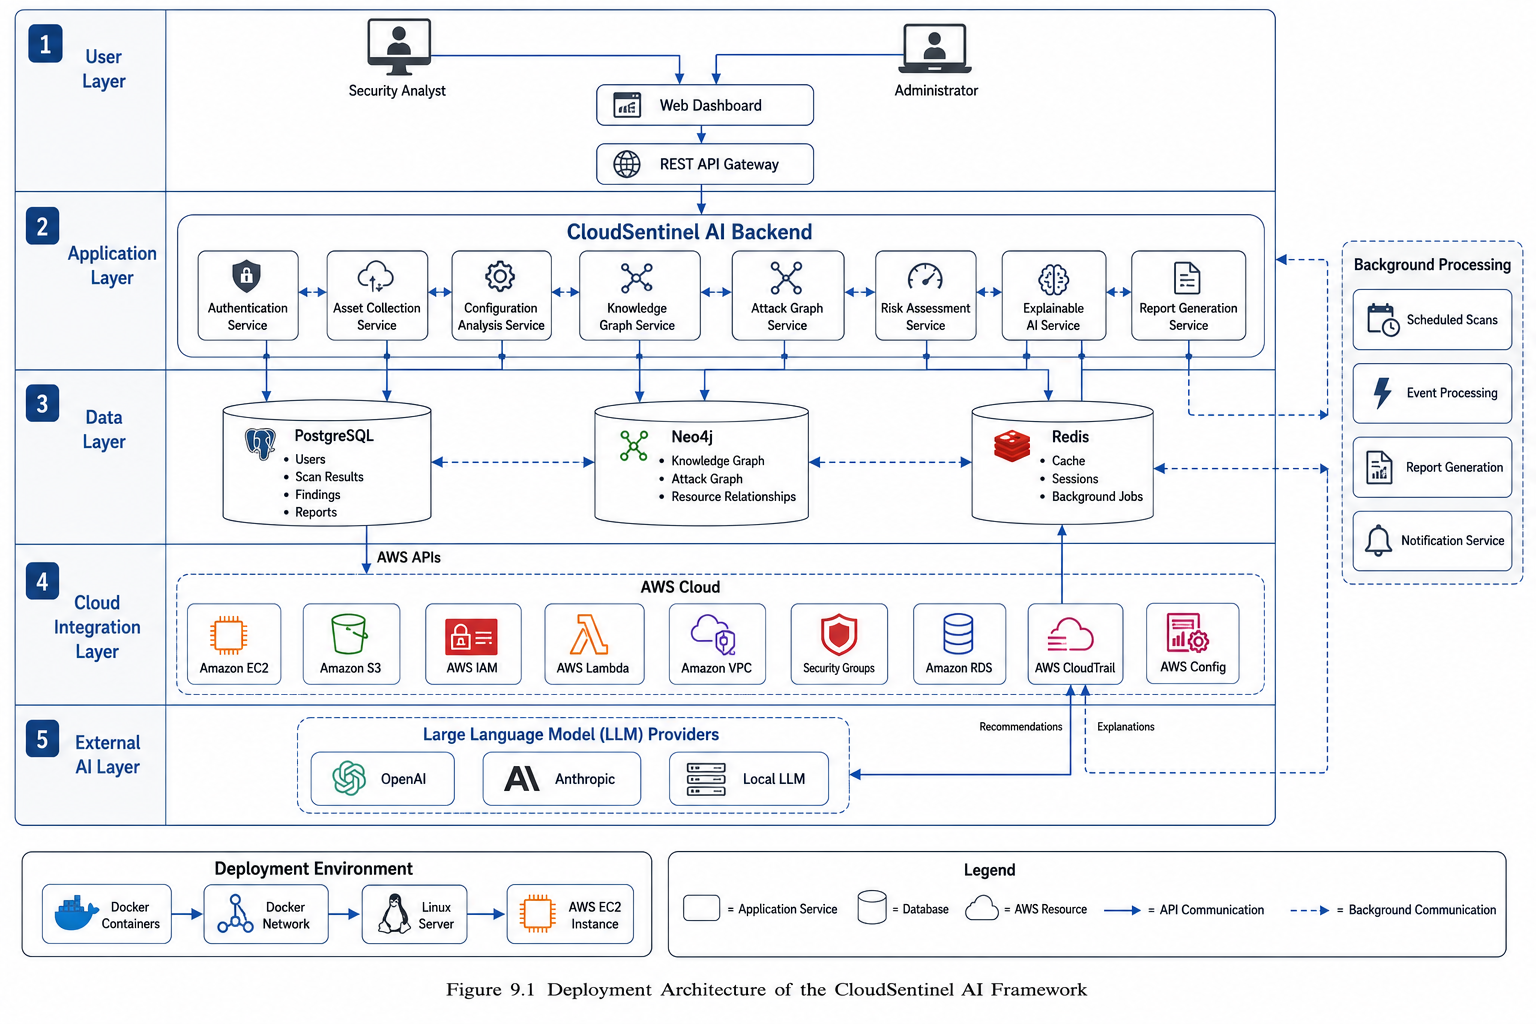
\includegraphics[width=0.9\textwidth,height=\textheight]{figures/image-9.1.png}
\caption{Knowledge Graph Representation.}\label{fig:9_1}
\end{figure}

\begin{figure}[H]
\centering
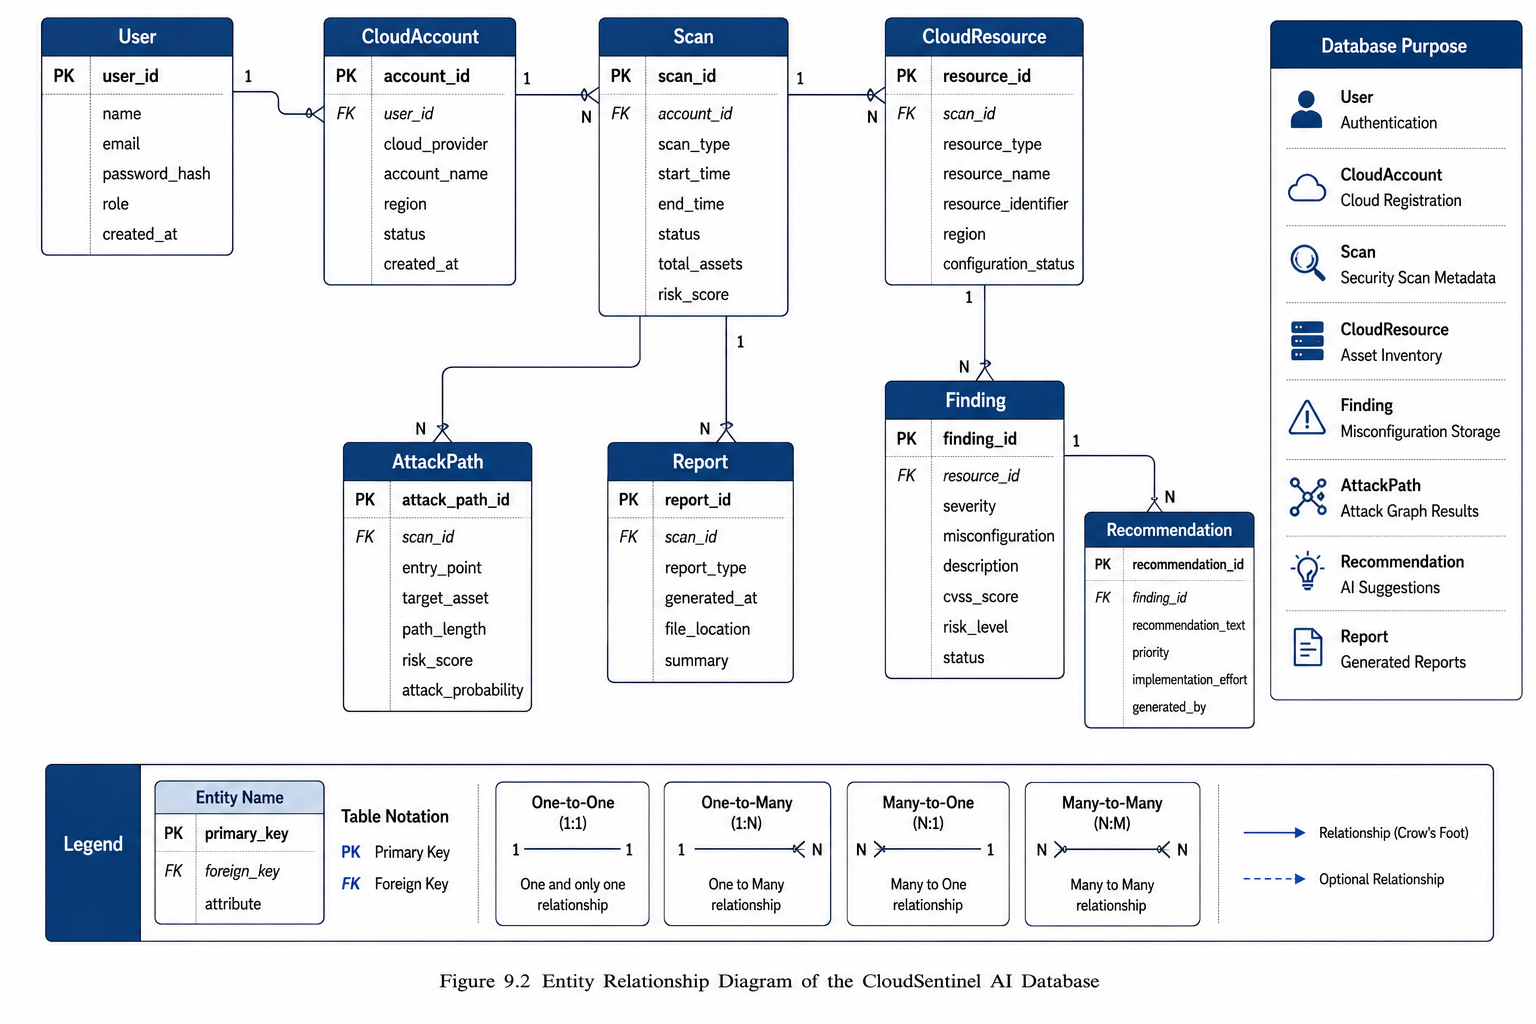
\includegraphics[width=0.9\textwidth,height=\textheight]{figures/image-9.2.png}
\caption{Attack Graph Generation Process.}\label{fig:9_2}
\end{figure}

\begin{figure}[H]
\centering
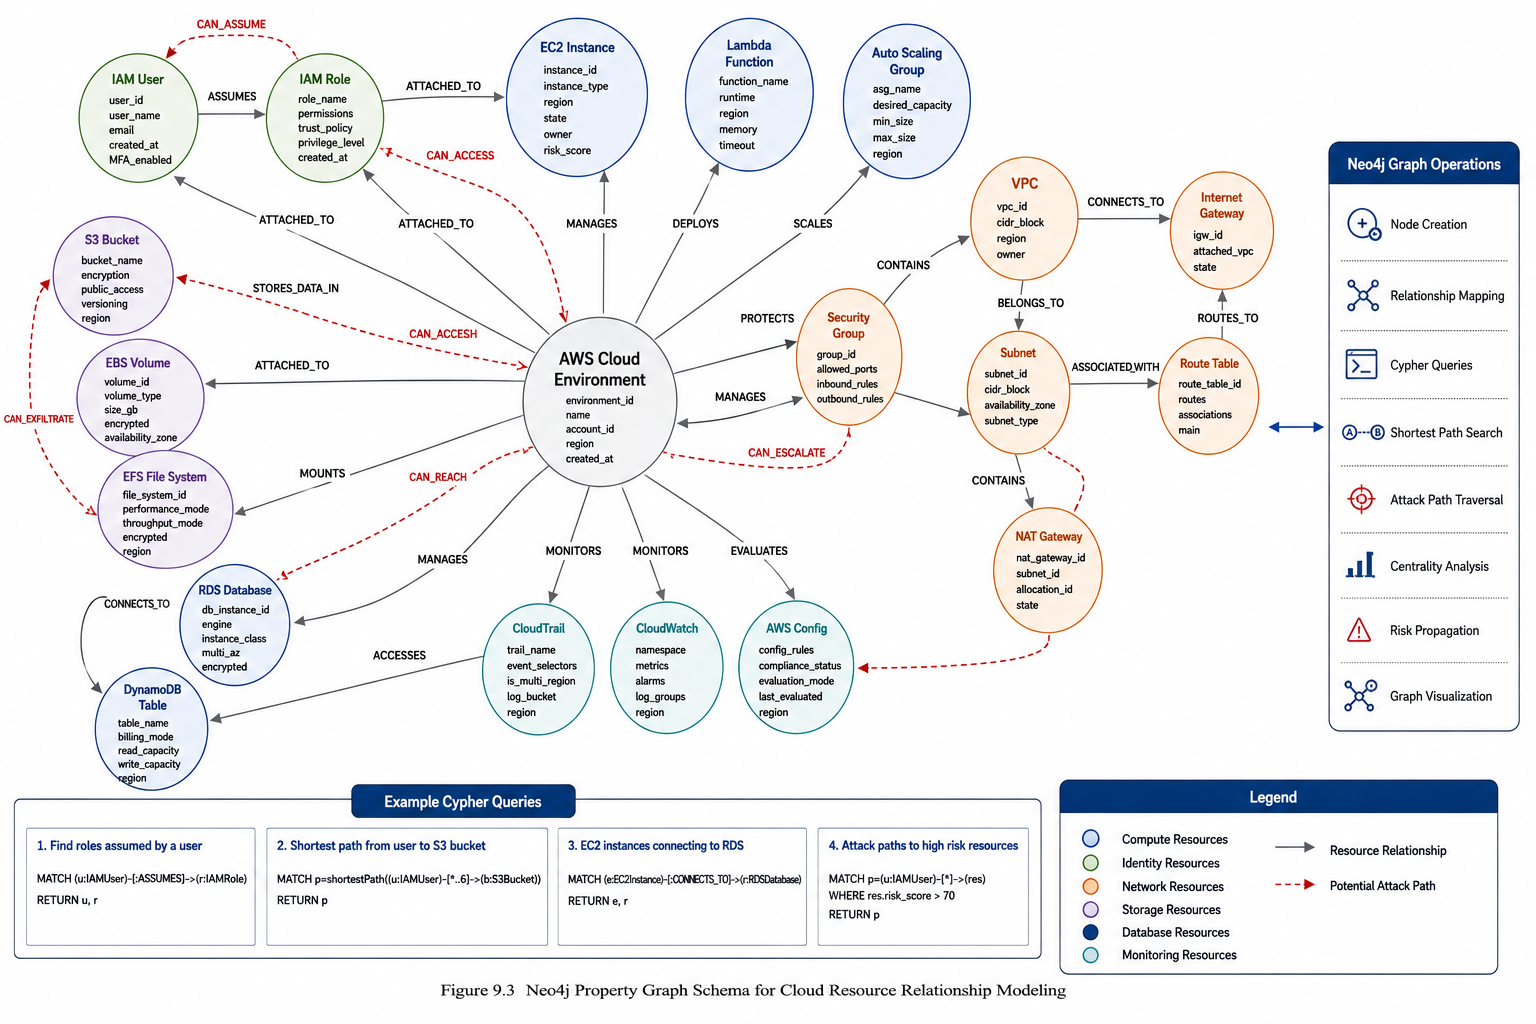
\includegraphics[width=0.9\textwidth,height=\textheight]{figures/image-9.3.png}
\caption{Context-Aware Risk Prioritization.}\label{fig:9_3}
\end{figure}
